\section{Introduction}
The project is a tribute to the to the popular '80s game: \textbf{Space Invaders} giving it our personal interpretation, in a 3D remake. At an early stage we made some design choices. The first one is the framework, Three.js in this case it seemed to fit perfectly our needs as well as being highly documented. \\
With the aim of addressing the difficulties of teamwork and to be open to further additions we have decided to use the MVC architectural pattern and other ones that will be described in this report taking advantage of the great work published on the blog hecodes.\\
The game will have four different modes:
\begin{enumerate}
\item Classic Arcade: \textit{Is the one similar to the original one;}
\item Classic Custom: \textit{Is similar to the previous one, but instead of levels you can choose the game parameters;}
\item Futuristic Arcade: \textit{It has the same dynamics of the classic mode, but the enemies have a more "realistic" movements;}
\item Futuristic Custom: \textit{Is similar to the previous one, but instead of levels you can choose the game parameters.}
\end{enumerate}
The \textit{"Arcade"} game modes involve the player in a session of 5 waves with escalating difficulties, while the \textit{"Custom"} ones regard uniquely a user-defined wave.\\
But before starting dive into the project in a more technical way, let's see how the main page will appear.
\begin{figure}[h!]
\begin{center}
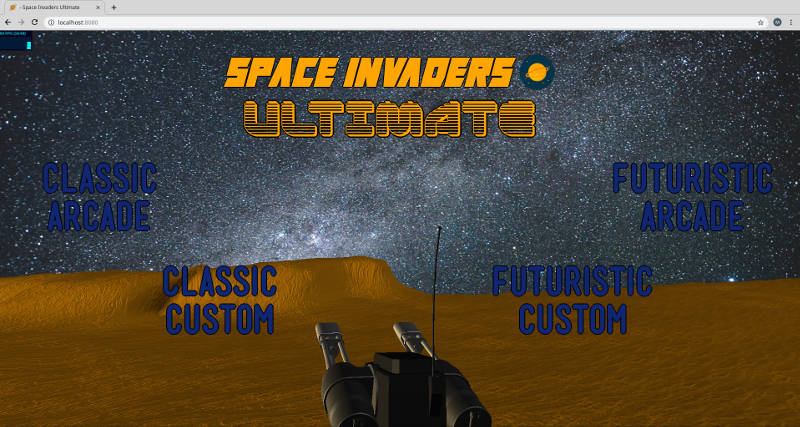
\includegraphics[scale=0.4]{images/siu-homepage.jpg}
\caption{The Animated HomePage of the final result}
\end{center}
\end{figure}